\section{Axiomatic Design}\label{sec:design}

The axiomatic design framework was developed in the late \(20^{th}\) century by Professor Nam P. Suh while at MIT
and the NSF~\cite{suh}.  This was in response to concern in the engineering community that \emph{design} was being
practiced almost exclusively as an ad-hoc creative endeavor with very little in the way of scientific discipline.
In the words of Professor Suh:
\begin{quote}
  \vspace{-\baselineskip}
  It [design] might have preceding the development of natural sciences by scores of centuries.  Yet, to this day,
  design is being done intuitively as an art.  It is one of the few technical areas where experience is more
  important than formal education~\cite{suh}.
\end{quote}
Professor Suh was not making these claims in an educational vacuum, but in the shadow of several recent major
design failures such as the Union Carbide plant disaster in India, nuclear power plant accidents at Three Mile
Island and Chernobyl, and the Challenger space shuttle O-ring failure.  Furthermore, Professor Suh asserts that
design-related issues resulting in production problems and operating failures were increasingly happening in
everything from consumer products to big-ticket items.  As a result, axiomatic design has been widely adopted by
companies to promote efficiency and accuracy in the design process, resulting in more reliable products and reduced
manufacturing costs~\cite{shirwaiker}.

The following sections provide an overview of axiomatic design as specified in detail by Professor
Suh~\cite{suh,suh2}, and summarized by Behdad, et al.~\cite{cavallaro,jahanbekam}.  Following the overview is a
description of how an algorithm proposed by this research can be a helpful tool to a designer using the axiomatic
design framework.

\subsection{Design}\label{sec:sub:design}

\emph{Design} is defined as the process by which it is determined \emph{what} needs to be achieved and then
\emph{how} to achieve it.  Thus, the decisions on what to do are just as important as how to do it.
\emph{Creativity} is the process by which experience and intuition are used to generate solutions to perceived
needs.  This includes pattern matching to and adapting existing solutions and synthesizing new solutions.  Thus,
creativity plays a vital role in design.  Since different designers may approach the same problem differently,
their level of creativity may lead to very different, yet plausible, solutions.  Therefore, there needs to be a
design-agnostic method for comparing different designs with the goal of selecting the best one.

This discussion will sound familiar to mathematicians, since creativity is a very important part of solving math
problems, and in particular, writing proofs.  Starting with the work of Peano in the \(19^{th}\) century, the field
of mathematics has established various tests on what constitutes a good proof.  For example:
\begin{itemize}
\item Does every conclusion result by proper implication from existing definitions, axioms, and previously proved
  conclusions?
\item Is direct proof, contrapositive proof, proof by contradiction, or proof by induction the best approach for a
  particular problem?
\item Do proofs by induction contain clear basic, assumptive, and inductive steps?
\item Are all subset and equality relationships properly proved via membership implication?
\item Are all necessary cases included and stated in a mutually exclusive manner?
\item Are degenerate cases sufficiently highlighted?
\item Are all equivalences proved in a proper circular fashion?
\item Are key and reused conclusions highlighted in lemmas?
\end{itemize}
In short, Professor Suh was looking for a similar framework for the more general concept of design.

\subsection{The Axiomatic Design Framework}\label{sec:sub:framework}

The \emph{best} design among a set of candidates is the design that exactly satisfies a clearly defined set of
needs and has the greatest probability of success.  In a desire not to hinder the creative element needed for
design, yet provide some methodology to distinguish bad designs from good designs from better designs, the diagram
in \figurename~\ref{fig:design} establishes the overall framework for axiomatic design.

\begin{figure}[H]
  \centering
  \scalebox{0.75}{
    \begin{tikzpicture}[>=latex',every text node part/.style={align=center}]
      \node (cn) [draw,terminal] at (0,0) {customer \\[-2ex] needs};
      \node (pd) [draw,process,right=of cn] {problem \\[-2ex] definition};
      \node (cp) [draw,process,right=2cm of pd] {creative \\[-2ex] process};
      \node (ap) [draw,process,right=2cm of cp] {analytical \\[-2ex] process};
      \node (uc) [draw,process,right=of ap] {ultimate \\[-2ex] check};
      \node (fd) [draw,terminal,right=of uc] {final \\[-2ex] design};
      \draw [->] (cn) -- (pd);
      \draw [->] (pd) -- node [auto] {FRs} (cp);
      \draw [->] (cp) -- node [auto] {candidate \\[-2ex] design} (ap);
      \draw [->] (ap) -- (uc);
      \draw [->] (uc) -- (fd);
      \draw [->] (ap) -- ($(ap) + (0,-1.5cm)$) -| (cp);
    \end{tikzpicture}
  }
  \caption{The axiomatic design framework.}
  \label{fig:design}
\end{figure}

Design starts with the desire to satisfy a set of clear \emph{customer needs}.  The term \emph{customer} refers to
any entity that expresses needs, and can be as varied as individuals, organizations, or society.  The designer, in
the \emph{problem definition} phase, determines how these customer needs will be met by generating a list of
\emph{functional requirements} (FRs).  It is this list of FRs that determines exactly \emph{what} is to be
accomplished.

Once the set of FRs has been determined, the designer begins the \emph{creative process} by mapping the FRs into
solutions that are embodied in so-called \emph{design parameters} (DPs).  The DPs contain all of the information on
\emph{how} the various FRs are satisfied: parts lists, drawings, specifications, etc.  The FRs exist in a
design-agnostic \emph{functional space} and the {\DP}s exist in a solution-specific \emph{physical space}.  It is
the designer's job to provide the most efficient mapping between the two spaces.  This process is represented by
\figurename~\ref{fig:mapping}.

\begin{figure}[H]
  \centering
  \begin{tikzpicture}[>=latex',every text node part/.style={align=center}]
    \node (fs) [draw,cloud] at (0,0) {FR1 \\ FR2 \\ FR3 \\ \vdots};
    \node [below=1ex of fs] {functional \\ space};
    \node (ps) [draw,cloud,right=1.5in of fs] {DP1 \\ DP2 \\ DP3 \\ \vdots};
    \node [below=1ex of ps] {physical \\ space};
    \draw [->] (fs) to [bend left=45] (ps);
    \draw [->] (fs) to [bend left=30] (ps);
    \draw [->] (fs) to [bend right=30] (ps);
    \draw [->] (fs) to [bend right=45] (ps);
    \draw [->] (fs) -- node [auto] {mapping} (ps);
  \end{tikzpicture}
  \caption{Mapping FRs to DPs.}
  \label{fig:mapping}
\end{figure}

Simple problems may require only one level of FRs; however, more complicated designs may require a hierarchial
structure of FRs from more general to more detailed requirements.  This type of design is often referred to as
\emph{top-down} design.  Each individual FR layer has its own DP mapping.  In fact, the mapping process on one
level should be completed prior to determining the FRs for the next level.  This is because DP choices on one level
may affect requirements on the next level.  For example, consider a FR related to a moving part in a design.  The
DP for this FR could specify that the part be moved manually or automatically.  Each choice would result in
different FRs for the actual mechanism selected by the DP.

The FR/DP mapping at each level in the design hierarchy is described by the \emph{design equation}, which is shown
in Equation~\ref{eqn:design}.
\begin{equation}
  \label{eqn:design}
  [\FR]=[\text{A}][\DP]
\end{equation}
The design equation is a matrix equation that maps a vector of \(m\) FRs to a vector of \(n\) DPs via an \(m\times
n\) design matrix A.  As will be shown, good designs require \(m=n\).  A full discussion of the design matrix
element values is beyond the scope of this research.  Instead, the following two values are used:
\[A_{ij}=\begin{cases}
X, & \FR_i\ \text{depends on}\ \DP_j \\
0, & \FR_i\ \text{does not depend on}\ \DP_j
\end{cases}\]

Since the FR/DP mapping is non-unique, there needs to be a method to compare different plausible designs so that
the best design can be selected as the final design.  Thus, the framework in \figurename~\ref{fig:design} includes
an \emph{analytical process}, where designs are judged by a set of axioms, corollaries, and theorems that specify
the properties common to all good designs.  Once the best design, according to this analysis, is selected, it
undergoes an \emph{ultimate check} to make sure that it sufficiently meets all of the customer's needs.  If so,
then that design is selected as the final design.

\subsection{The Axioms}\label{sec:sub:axioms}

The analytical process is based on two main axioms: the independence axiom and the information axiom.  This section
describes these axioms and their related corollaries and theorems.

The independence axiom~\cite{suh} imposes a restriction on the FR/DP mapping:

\begin{axiom}[The Independence Axiom]
  \label{axm:independence}
  An optimal design always maintains the independence of the FRs.  This means that the FRs and DPs are related in
  such a way that a specific DP can be adjusted to satisfy its corresponding FR without affecting other FRs.
\end{axiom}

The ideal case is when the design matrix is a diagonal matrix, and so each FR is mapped to and is satisfied by
exactly one DP.  This is referred to as an \emph{uncoupled} design, which is demonstrated in
\figurename~\ref{fig:uncoupled}.  Uncoupled designs completely adhere to the independence axiom.

\begin{figure}[H]
  \begin{equation*}
    \begin{bmatrix}
      \FR1 \\ \FR2 \\ \FR3
    \end{bmatrix}=\begin{bmatrix}
    X & 0 & 0 \\
    0 & X & 0 \\
    0 & 0 & X
    \end{bmatrix}\begin{bmatrix}
      \DP1 \\ \DP2 \\ \DP3
    \end{bmatrix}
  \end{equation*}
  \vspace{-\baselineskip}
  \caption{An uncoupled design.}
  \label{fig:uncoupled}
\end{figure}

The next best situation is when the design matrix is a lower-triangular matrix.  The idea is to finalize the first
DPs before moving on to the later DPs.  Thus, \(\text{DP}_i\) can be adjusted without affected \(\FR_1\) through
\(\FR_{i-1}\).  This is referred to as a \emph{decoupled} design, which is demonstrated in
\figurename~\ref{fig:decoupled}.  Although decoupled designs do not completely adhere to the independence axiom,
they may be reasonable compromises in designs that address complex problems.

\begin{figure}[H]
  \begin{equation*}
    \begin{bmatrix}
      \FR1 \\ \FR2 \\ \FR3
    \end{bmatrix}=\begin{bmatrix}
    X & 0 & 0 \\
    X & X & 0 \\
    X & X & X
    \end{bmatrix}\begin{bmatrix}
      \DP1 \\ \DP2 \\ \DP3
    \end{bmatrix}
  \end{equation*}
  \vspace{-\baselineskip}
  \caption{A decoupled design.}
  \label{fig:decoupled}
\end{figure}

The worst solution is a non-triangular matrix, where every change in a DP affects multiple FRs in an unconstrained
fashion.  This is referred to as a \emph{coupled} design, which is demonstrated in \figurename~\ref{fig:coupled}.
Coupled designs are in complete violation of the independence axiom and generally should be decoupled by reworking
the FRs or by adding additional DPs.

\begin{figure}[H]
  \begin{equation*}
    \begin{bmatrix}
      \FR1 \\ \FR2 \\ \FR3
    \end{bmatrix}=\begin{bmatrix}
    X & X & X \\
    X & X & X \\
    X & X & X
    \end{bmatrix}\begin{bmatrix}
      \DP1 \\ \DP2 \\ \DP3
    \end{bmatrix}
  \end{equation*}
  \vspace{-\baselineskip}
  \caption{A coupled design.}
  \label{fig:coupled}
\end{figure}

Unfortunately, adding additional DPs runs counter to the second axiom: the information axiom~\cite{suh}.

\begin{axiom}[The Information Axiom]
  The best design is a functionally uncoupled design that has the minimum information content.
\end{axiom}

The amount of \emph{Information} contained in a particular DP is inversely related to the probability that the DP
can successfully satisfy its corresponding FR(s) by Equation~\ref{eqn:info}.
\begin{equation}
  \label{eqn:info}
  I=\log_2\left(\frac{1}{p}\right)
\end{equation}
where \(p\) is the probability of success and \(I\) is measured in bits.  This probability must take into
consideration such things as tolerances, ease of manufacture, failure rates, etc.  The information content of a
design is then the sum of the information content of its individual DPs.

From these two axioms come the following seven corollaries~\cite{suh}:
\begin{corollary}
  \label{cor:decouple}
  Decouple or separate parts or aspects of a solution if the FRs are coupled or become interdependent in the
  designs proposed.
\end{corollary}
\begin{corollary}
  \label{cor:minfrs}
  Minimize the number of FRs.
\end{corollary}
\begin{corollary}
  \label{cor:integrate}
  Integrate design features in a single physical part if FRs can be independently satisfied in the proposed
  solution.
\end{corollary}
\begin{corollary}
  \label{cor:standard}
  Use standardized or interchangeable parts if the use of these parts is consistent with the FRs.
\end{corollary}
\begin{corollary}
  \label{cor:shapes}
  Use symmetrical shapes and/or arrangements if they are consistent with the FRs.
\end{corollary}
\begin{corollary}
  \label{cor:tolerance}
  Specify the largest allowable tolerance in stating FRs.
\end{corollary}
\begin{corollary}
  \label{cor:uncoupled}
  Seek an uncoupled design that requires less information than coupled designs in satisfying a set of FRs.
\end{corollary}

The theorems that arise from these axioms and corollaries are used to prove that an optimal design results from a
square design matrix.  In other words, the number of FRs should be equal to the number of DPs.  First, consider the
case where there are more FRs than DPs.  This forces a single DP to be mapped to multiple FRs.  Otherwise, some FRs
cannot be satisfied by the DPs.  This result is stated in Theorem~\ref{thm:frgtdp}~\cite{suh}.

\begin{theorem}
  \label{thm:frgtdp}
  When the number of DPs is less that the number of FRs, either a coupled design results or the FRs cannot be
  satisfied.
\end{theorem}

A possible solution to this problem is given by Theorem~\ref{thm:adddp}~\cite{suh}.
\begin{theorem}
  \label{thm:adddp}
  A coupled design due to more FRs than DPs can be decoupled by adding new DPs if the additional DPs result in a
  lower triangular design matrix.
\end{theorem}

An example is show in \figurename~\ref{fig:dcexample}.  Note that the addition of DP3 results in a decoupled design.

\begin{figure}[H]
  \[\begin{bmatrix}
  \FR1 \\ \FR2 \\ \FR3
  \end{bmatrix}=\begin{bmatrix}
  X & 0 \\
  X & X \\
  X & X \\
  \end{bmatrix}\begin{bmatrix}
    \DP1 \\ \DP2 \\
  \end{bmatrix}\implies\begin{bmatrix}
  \FR1 \\ \FR2 \\ \FR3
  \end{bmatrix}=\begin{bmatrix}
  X & 0 & 0 \\
  X & X & 0 \\
  X & X & X \\
  \end{bmatrix}\begin{bmatrix}
    \DP1 \\ \DP2 \\ \DP3
  \end{bmatrix}\]
  \vspace{-\baselineskip}
  \caption{Decoupling a design by adding DPs.}
  \label{fig:dcexample}
\end{figure}

Next, consider the case where the number of FRs is less than the number of DPs.  Assuming that the design is not
coupled, this means that either a DP exists that does not address any FRs or multiple DPs exist that address a
single FR and hence can be integrated into a single DP.  Such a design is called a \emph{redundant} design.  This
is addressed by Theorem~\ref{thm:frltdp}~\cite{suh}.

\begin{theorem}
  \label{thm:frltdp}
  When there are less FRs than DPs then the design is either coupled or redundant.
\end{theorem}

Finally, the previous three theorems lead to the conclusion in Theorem~\ref{thm:freqdp}~\cite{suh}.

\begin{theorem}
  \label{thm:freqdp}
  In an ideal design, the number of FRs is equal to the number of DPs.
\end{theorem}

\subsection{Part Consolidation}\label{sec:sub:parts}

One particularly important design parameter is the number of parts in a product design.  According to Professor
Suh:
\begin{quote}
  \vspace{-\baselineskip}
  Poorly designed products often cost more because they use more materials or parts than do well-designed products.
  They are often difficult to manufacture and maintain~\cite{suh}.
\end{quote}
Decreasing the number of parts in a design while maintaining the independence of the FRs is consistent with
Corollary \ref{cor:integrate} and lowers the information content of the design.  In fact, Tang, et al.~\cite{tang}
describe how part consolidation reduces the weight and complexity of a final product while boosting reliability and
reducing cost.

An informative example of part consolidation is the combination can/bottle opener shown in
\figurename~\ref{fig:opener}.  The design of this handy utensil has two FRs, shown in \tablename~\ref{tab:opener}.
Both FRs are consolidated into a single part, yet remain independent as long as there is no desire to open a can
and a bottle simultaneously (although that would be a popular trick around a campfire).

\begin{figure}[H]
  \centering
  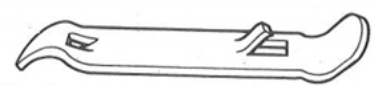
\includegraphics{opener}
  \caption{A part consolidation example.}
  \label{fig:opener}
\end{figure}

\begin{table}[H]
  \caption{Opener Functional Requirements}
  \label{tab:opener}
  \centering
  \begin{tabular}{|c|l|}
    \hline
    FR1 & Open beverage cans \\
    \hline
    FR2 & Open beverage bottles \\
    \hline
  \end{tabular}
\end{table}

The goal of this research is to provide designers with a tool that they can use to determine the minimum number of
parts required to realize a particular design at a particular level in a FR/DP hierarchy.  The designer is required
to construct a graph whose vertices are the FRs and whose edges indicate that the endpoint FRs need to be realized
by separate parts due to specific design constraints.  How these edges are actually determined is beyond the scope
of this research.  Adjacent FRs are candidates for part consolidation.  The goal is to find the chromatic number of
the resulting graph, which corresponds to the minimum number of parts.

To be a viable tool, a computer program must be able to deliver an answer in a reasonable amount of time.
Unfortunately, finding the chromatic number of a graph is known to be an NP-hard problem~\cite{mcdiarmid} and so
the time required to find a solution grows exponentially with the number of FR vertices and edges in the graph.
Thus, an algorithm is proposed with improved runtime complexity that can be run on a computer in order to provide a
designer with an answer in a reasonable amount of time.  Designs with different minimum part requirements can then
be compared during the analytical process as part of the overall process of selecting the best design.
